\documentclass{article}
\usepackage[landscape]{geometry}
\usepackage{url}
\usepackage{multicol}
\usepackage{amsmath}
\usepackage{esint}
\usepackage{amsthm}
\usepackage{amsfonts}
\usepackage{booktabs}
\usepackage{tikz}
\usetikzlibrary{shapes,backgrounds,calc,patterns,positioning}
\usepackage{pgfplots}
\usepgflibrary{shadings}
\usepackage{amsmath,amssymb}
\usepackage{subcaption}
\usepackage[english]{babel}
\usepackage{enumitem}
\usetikzlibrary{decorations.markings}


\usepackage{colortbl}
\usepackage{xcolor}
\usepackage{mathtools}
\usepackage{amsmath,amssymb}
\usepackage{enumitem}
\makeatletter

\definecolor{horange}{HTML}{f58026}

\newcommand*\bigcdot{\mathpalette\bigcdot@{.5}}
\newcommand*\bigcdot@[2]{\mathbin{\vcenter{\hbox{\scalebox{#2}{\(\m@th#1\bullet\)}}}}}
\makeatother

\newenvironment{solution}%
    {\textit{Solution.}}

    \newcommand{\sol}[1]{
        \begin{solution}
            #1
        \end{solution}
    }

\title{Discrete Exam 2 Note Sheets}
\usepackage[utf8]{inputenc}

\advance\topmargin-.8in
\advance\textheight
3in
\advance\textwidth3in
\advance\oddsidemargin-1.40in
\advance\evensidemargin-1.45in
\parindent0pt
\parskip1pt
\newcommand{\hr}{\centerline{\rule{3.5in}{1pt}}}

% Natural Numbers 
\newcommand{\N}{\ensuremath{\mathbb{N}}}

% Whole Numbers
\newcommand{\W}{\ensuremath{\mathbb{W}}}

% Integers
\newcommand{\Z}{\ensuremath{\mathbb{Z}}}

% Rational Numbers
\newcommand{\Q}{\ensuremath{\mathbb{Q}}}

% Real Numbers
\newcommand{\R}{\ensuremath{\mathbb{R}}}

% Complex Numbers
\newcommand{\C}{\ensuremath{\mathbb{C}}}

\newcommand{\brackett}[1]{\left\langle #1 \right\rangle}

\newcommand{\norm}[1]{\left\lVert \mathbf{#1}\right\rVert}

\newcommand{\dydx}{\tfrac{dy}{dx}}
\newcommand{\dxdy}{\tfrac{dx}{dy}}
\newcommand{\dydt}{\tfrac{dy}{dt}}
\newcommand{\dxdt}{\tfrac{dx}{dt}}
\newcommand{\dzdt}{\tfrac{dz}{dt}}


\newcommand{\cost}{\cos(t)}
\newcommand{\sint}{\sin(t)}
\newcommand{\tant}{\tan(t)}
\newcommand{\p}{\partial}

% 
\newcommand{\barNotationT}[1]{\bigg|_{t = #1}}

\newcommand{\mb}[1]{\mathbf{#1}}

\newcommand{\imb}{\mb{i}}
\newcommand{\jmb}{\mb{j}}
\newcommand{\kmb}{\mb{k}}
\newcommand{\rmb}{\mb{r}}
\newcommand{\umb}{\mb{u}}

\newcommand{\mbi}{\mathbf{i}}
\newcommand{\mbj}{\mathbf{j}}
\newcommand{\mbk}{\mathbf{k}}
\newcommand{\mbr}{\mathbf{r}}

\newcommand{\vecfuc}[2]{\mb{#1}(#2)}
\newcommand{\dvecfuc}[2]{\mb{#1}'(#2)}
\newcommand{\normdvecfuc}[2]{||\mb{#1}'(#2)||}

\DeclareMathOperator{\arccot}{arccot}
\DeclareMathOperator{\arcsec}{arcsec}
\DeclareMathOperator{\arccsc}{arccsc}

\usepackage{titlesec}

\newcommand{\mysqrt}[1]{%
  \mathpalette\foo{#1}%
}
\newcommand{\dmysqrt}[1]{%
  \mathpalette\foodisplay{#1}%
}

% !TeX spellcheck = off
\newcommand{\foo}[2]{%
  % #1: math style, #2: content
  \sbox0{$#1\sqrt{#2}$}% Measure the size of the standard sqrt in the current style
  \begin{tikzpicture}[baseline=(sqrt.base)]
    \node[inner sep=0, outer sep=0] (sqrt) {$#1\sqrt{#2}$}; % Use the current math style
    \draw([yshift=-0.045em]sqrt.north east) -- ++(0,-0.5ex); % Draw the tick
  \end{tikzpicture}%
}
% !TeX spellcheck = off
\newcommand{\foodisplay}[2]{%
  % #1: math style, #2: content
  \sbox0{$#1\sqrt{#2}$}% Measure the size of the standard sqrt in the current style
  \begin{tikzpicture}[baseline=(sqrt.base)]
    \node[inner sep=0, outer sep=0] (sqrt) {$\displaystyle\sqrt{#2}$}; % Force displaystyle
    \draw[line width=0.4pt] ([yshift=-0.044em]sqrt.north east) -- ++(0,-0.5ex); % Draw the tick
  \end{tikzpicture}%
}

\setlist[enumerate,1]{left=0pt}
\setlist[enumerate,2]{left=-10pt}


\begin{document}





















\begin{center}{\huge{\textbf{Multivariable Calculus Exam 4}}}\\
\end{center}
\begin{multicols*}{2}

    \tikzstyle{mybox} = [draw=black, fill=white, very thick,
    rectangle, rounded corners, inner sep=5pt, inner ysep=10pt]
    \tikzstyle{innerbox} = [draw=black, fill=gray!20, thick,
    rectangle, rounded corners, inner sep=5pt, inner ysep=10pt]
    \tikzstyle{fancytitle} =[fill=black, text=white, font=\bfseries]

    %------------ Measures of Center ---------------

    \begin{tikzpicture}
        \node [mybox] (box){%
            \begin{minipage}{0.46\textwidth}

                \begin{itemize}
                    \item \textbf{Slope:} \& \textbf{Equation} \(\dydx = \frac{dy/dt}{dx/dt};\) \& \(y = \frac{dy}{dx}(x - x(t_{0})) + y(t_{0})\). For example, the curve defined by \(x(t) = 3t^{2} - 8t + 1\) and \(y(t) = e^{-t^{2}}\), for \(0 \leq t \leq 2\). Finding the equation at \(t = 1\), we get:

                          \sol{
                          \(\frac{dy/dt}{dx/dt} = \frac{-2te^{-t^{2}}}{6t - 8}\), then we plug in \(t = 1\):
                          \(x(1) = -4\), \(y(1) = e^{-1}\), and our slope: \(\frac{-2e^{-1}}{6 - 8} = e^{-1}\). Giving the equation \(y = e^{-1}(x + 4) + e^{-1}\).
                          }
                    \item \textbf{Concavity:} \(\frac{d^{2}y}{dx^{2}}\big|_{t_{0}} = \frac{\frac{d}{dt}(dy/dx)}{dx/dt}\big|_{t_{0}}\). Remember, + \(\Rightarrow\) concave up.
                    \item \textbf{Area Under a Curve:} \(\int_{t_{a}}^{t_{b}} y(t) \frac{dx}{dt} \, dt\).
                    \item \textbf{Arc Length:} \(\int_{t_{a}}^{t_{b}} \mysqrt{(\frac{dx}{dt})^{2} + (\frac{dy}{dt})^{2}} \, dt\).
                    \item \textbf{Surface Area:} \(\int_{t_{a}}^{t_{b}} 2\pi y(t) \mysqrt{(\frac{dx}{dt})^{2} + (\frac{dy}{dt})^{2}} \, dt\).
                    \item \textbf{Direction:} \(P = (x_{1},y_{1})\) and \(Q = (x_{2},y_{2})\): \(\mathbf{PQ} = \langle x_{2}-x_{1},y_{2}-y_{1}\rangle\).
                    \item \textbf{Vector Sum:} \(\mathbf{u} + \mathbf{v} = \langle u_{1} + v_{1}, u_{2} + v_{2}\rangle\).
                    \item \textbf{Magnitude:} \(\norm{u} = \mysqrt{u_{1}^{2} + u_{2}^{2}}\).
                    \item \textbf{Dot Product:} \(\mathbf{u} \cdot \mathbf{v} = u_{1}v_{1} + u_{2}v_{2}\).
                    \item To \textbf{Normalize} a vector, divide it by its magnitude \(\mb{v} = \brackett{x,y,z}\), then \(\mb{u} = \frac{1}{\norm{\mb{v}}}\mb{v} = \brackett{\frac{x}{\norm{v}},\frac{y}{\norm{v}}, \frac{z}{\norm{v}}}\). \(\therefore\mb{u} :=\) \textbf{Unit Vector} in direction of \(\mb{v}\).
                    \item \textbf{Projection:} \(\text{proj}_{\mathbf{v}}\mathbf{u} = \left(\frac{\mathbf{u} \cdot \mathbf{v}}{\norm{v}^{2}}\right)\mathbf{v}.\)
                    \item \textbf{Cross product:} \(\mathbf{u} \times \mathbf{v} = \brackett{u_{2}v_{3} - u_{3}v_{2}, \ u_{3}v_{1} - u_{1}v_{3}, \ u_{1}v_{2} - u_{2}v_{1}}.\).
                    \item \textbf{Symmetric Equation:} \(\frac{x - x_{0}}{a} = \frac{y - y_{0}}{b} = \frac{z - z_{0}}{c}\). E.g., For the points: \(R = (4,-6,1)\) and \(S = (1,2,3)\): \(\frac{x - R_{1}}{S_{1} - R_{1}} = \frac{y - R_{2}}{S_{2} - R_{2}} = \frac{z - R_{3}}{S_{3} - R_{3}}\) or \(\frac{x - 4}{-3} = \frac{y + 6}{8} = \frac{z - 1}{2}\).
                    \item If \((x_{0},y_{0},z_{0})\) is a point on a plane, the \textbf{Scalar Equation} would be: \(\brackett{x - x_{0}, y - y_{0}, z - z_{0}} \cdot \brackett{a,b,c} = 0 \Longrightarrow a(x - x_{0}) + b(y - y_{0}) + c(z - z_{0}) = 0\).
                    \item To \textbf{Parameterize} an equation such as \(y = x^{3} - 4x + 1\) we can let \(x = t\) and \(y = t^{3} - 4t + 1\). This allows us to write the equation as \(\mb{r}(t) = \brackett{t,t^{3} - 4t + 1}\).
                    \item \textbf{Velocity Vector:} \(\mb{v}(t) = \dvecfuc{r}{t}\).
                    \item \textbf{Unit Tangent Vector:} \(\mb{T}(t) = \frac{\mb{v}(t)}{\norm{\mb{v}(t)}}\).
                    \item \textbf{Area:} \(\iint_{D} 1 \, dA\), where \(D\) is the region in the \(xy\)-plane over which we are integrating. \(\int_{a}^{b} \int_{c}^{d} f(x,y) \, dy \, dx\).
                \end{itemize}

            \end{minipage}
        };
        %------------ Continuous Random Variable and Distributions Header ---------------------
        \node[fancytitle, right=10pt] at (box.north west) {Terms and Formulas};
    \end{tikzpicture}




    %------------ Summarizing Main Features of f(x) ---------------
    \begin{tikzpicture}
        \node [mybox] (box){%
            \begin{minipage}{0.46\textwidth}
                \begin{itemize}
                    \item \textbf{Second derivative test:} \(\Delta = f_{xx}f_{yy} - (f_{xy})^{2}\). If \(\Delta > 0\) and \(f_{xx} > 0\), then \(f\) has a local min. If \(\Delta > 0\) and \(f_{xx} < 0\), then \(f\) has a local max. If \(\Delta < 0\), then \(f\) has a saddle point. If \(\Delta = 0\), then the test is inconclusive.
                \end{itemize}
                \textbf{Curvature:} \(\kappa = \frac{\| \mb{T}'(t)\| }{ \|\mb{r}'(t)\| }\); for \(\R^{3}\): \(\kappa = \frac{ \|\mb{r}'(t) \times \mb{r}''(t)\| }{ \|\mb{r}'(t)||^{3}}\); if \(y = f(x)\): \(\kappa = \frac{|y''(x)|}{[1 + (y'(x)^{2})]^{3/2}}\)
                \begin{enumerate}
                    \item Find an equation in scalar form of the plane which passes through \((-2,7,1)\) and is perpendicular to the planes \(3x + y - z = 0 \) and \(-2x - y + 5z + 1 = 0\) [Hint: Think about what the relationship among the various normal vectors must be.]

                          \sol{
                              For the plane to be perpendicular to a given plane, its normal vector must lie in that given plane. Hence, our normal vector must be orthogonal to both \(\brackett{3,1,-1}\) and \(\brackett{-2,-1,5}\). Thus, we can take the cross product of these two vectors to get our normal vector: \(\brackett{3,1,-1} \times \brackett{-2,-1,5} =  \brackett{4,-13,-1}.\)
                              With our normal vector found, we can plug in our point to get our scalar equation: \(4(x + 2) - 13(y - 7) - (z - 1) = 0\).
                          }
                    \item Write, in general equation form, an equation of the plane which contains the three points \(P = (2,7,3)\), \(Q = (-5,0,1)\), and \(R = (-3,1,2)\).

                          \sol{
                              Find \(\mb{PQ} = \brackett{-7,-7,-2} \text{ and } \mb{PR} = \brackett{-5,-6,-1}.\)
                              Then, we find \(\mb{n}\) by solving for the cross product.
                              With \(\mb{n}\) (\(\brackett{-5,3,7}\)), we get the general formula: \(\boxed{-5(x - 2) + 3(y - 7) + 7(z - 3) = 0.}\) where the numbers inside come from \(P\). This can be directly translated to symmetric form by just plugging into the equation:
                              \(\frac{x - x_{0}}{n_{x}} = \frac{y - y_{0}}{n_{y}} = \frac{z - z_{0}}{n_{z}}\) where \(n_{x}, n_{y}, n_{z}\) are the components of the normal vector and \(x_{0}, y_{0}, z_{0}\) are the coordinates of point \(P\).
                          }

                    \item Find an equation, in symmetric form, of the line of intersection between the planes \(2x + y - z + 4 = 0\) and \(x - y + 3z = 1\).

                          \sol{
                              Choose parameter \(t = z\). From \(2x + y - z + 4 = 0 \Rightarrow y = -2x + z - 4\). Plug into \(x - y + 3z = 1\): \(x - (-2x + z -4) + 3z = 1 \implies 3x + 2z + 4 = 1 \implies 3x + 2z = -3 \implies x = -1 - \frac{2}{3}z\). Then, \(x = -1 - \frac{2}{3}z\), \(y = -2 + \frac{7}{3}z\), and \(z = z\). Set \(z = -3t\) (so the denominators clear): \(x = -1 + 2t\), \(y = -2 - 7t\), \(z = -3t\). This gives: \(\frac{x + 1}{2} = \frac{y + 2}{-7} = \frac{z}{-3}\).
                          }
                \end{enumerate}
            \end{minipage}
        };
        %------------ Summarizing Main Features of f(x) ---------------------
        \node[fancytitle, right=10pt] at (box.north west) {Derivative Test, Curvature, and Practice Set \# 1};
    \end{tikzpicture}



    \begin{tikzpicture}
        \node [mybox] (box){%
            \begin{minipage}{0.46\textwidth}
                \begin{enumerate}
                    \item Write, in scalar form, an equation of the plane which contains the point \((5,2,1)\) and the line given by \(x + 2 = \dfrac{y}{4} = \dfrac{z - 5}{2}\).

                          \sol{
                              We start by parametrizing the line with common parameter \(t\):
                              \(x + 2 = t \Rightarrow x = t - 2\), \(\frac{y}{4} = t \Rightarrow y = 4t\), and \(\frac{z - 5}{2} = t \Rightarrow z = 2t + 5\). This yields \((x,y,z) = (-2,0,5) + t(1,4,2)\). Thus, the line passes through \((-2,0,5)\) and has the direction vector \(\mb{v}_{1} = \brackett{1,4,2}\). We can form a second vector \(\mb{v}_{2}\) by taking the difference between the given point and a point on the line: \(\mb{v}_{2} = (5,2,1) - (-2,0,5) = \brackett{7,2,-4}\). Then, we find the cross product to get the normal vector. With the normal, we find the scalar form to be \(-20(x + 2) + 18y - 26(z - 5) = 0\).
                          }
                    \item  Find total distance of a particle over a time period \([0,3\pi]\) for the position equation \(\mb{r}(t) = \brackett{\sin(t), t, 3t}\). \\
                          \sol{
                              \(\displaystyle \int_{0}^{3\pi} \|\dvecfuc{r}{t} \| \, dt = \int_{0}^{3\pi} \mysqrt{\cos^{2}(t) + 1 + 9} \, dt = 9.709\).
                          }
                    \item Use curvature to find the equation of the osculating circle at the planar curve \(y = x^{3} - 4x + 1\) at \(x = 1\).

                          \sol{
                              First, we need to find the curvature of the curve at \(x = 1\). We start by finding the first and second derivatives of the function: \(y'(x) = 3x^{2} - 4\), \(y''(x) = 6x\). Plugging in for \(x = 1\), we get \(y(1) = -2\), \(y'(1) = -1\), and \(y''(1) = 6\). With these values, we can find the curvature: \(\kappa = \frac{6}{(1 + (-1)^{2})^{3/2}} = \frac{3\mysqrt{2}}{3}\).
                              With the curvature, we can find the radius of the osculating circle: \(R = \frac{1}{\kappa} = \frac{\mysqrt{2}}{3}\). Plug in \(x = 1\) to find the center with the unit normal vector: \(\mb{N} = \frac{(-y',1)}{\mysqrt{1 + (y')^{2}}} = \frac{(1,1)}{\mysqrt{2}}\). The center can be found by moving our point \(P(1,-2)\) the distance \(R\) along the unit normal vector: \(C = P + R\mb{N} = (1,-2) + \frac{\mysqrt{2}}{3}\frac{(1,1)}{\mysqrt{2}} = \left(\frac{4}{3},-\frac{5}{3}\right)\). This gives the equation for the osculating circle: \(\left(x - \frac{4}{3}\right)^{2} + \left(y + \frac{5}{3}\right)^{2} = \frac{2}{9}\).
                          }
                    \item Find an equation of the tangent plane to \(f(x,y) = x^{2}y - \mysqrt{x} + y\) at the point \((3,1)\). \\
                          \sol{
                              Solve for \(f_{x}(x,y)\), then \(f_{x}(3,1)\), and \(f_{y}(x,y)\), then \(f_{y}(3,1)\) to get the values of the partial derivatives at the point \((3,1)\):
                              \begin{align*}
                                  z & = f(3,1) + f_{x}(3,1)(x - 3) + f_{y}(3,1)(y - 1)   \\
                                    & = 7 + \tfrac{23}{4}(x - 3) + \tfrac{35}{4}(y - 1).
                              \end{align*}
                          }
                    \item What is the angle between \(\mb{u} = \brackett{6,2,-5}\) and \(\mb{v} = \brackett{-4,1,-7}\)?

                          \sol{
                              \(\theta = \cos^{-1}\left(\frac{\mb{u} \cdot \mb{v}}{\norm{\mb{u}}\norm{\mb{v}}}\right) = \cos^{-1}\left(\frac{13}{\mysqrt{65}\mysqrt{66}}\right) = 0.198\) rads.
                          }
                \end{enumerate}

            \end{minipage}
        };
        %------------ Measures of Center Header ---------------------
        \node[fancytitle, right=10pt] at (box.north west) {Practice Set \# 2};
    \end{tikzpicture}

    \begin{tikzpicture}
        \node [mybox] (box){%
            \begin{minipage}{0.46\textwidth}

                \begin{multicols}{2}
                    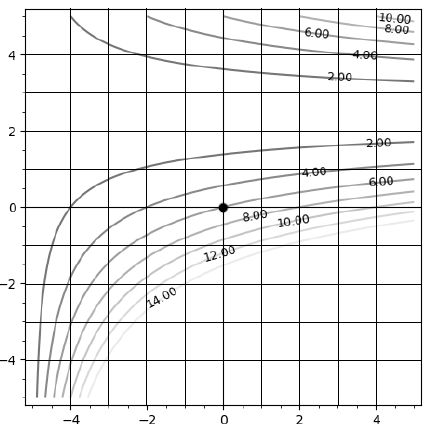
\includegraphics[width=6cm]{Images/contour_plot.png}
                    Determine the sign (\(+, \, -, \, 0\)) for each of the following partial derivatives.
                    \begin{enumerate}
                        \item \(f_{x}(0,0)\) \\
                              We see \(f(0,0) \approx 6\). As we move right (positive \(x\)), \(f\) increases, toward value 8. Thus, \(+\).
                        \item \(f_{y}(0,0)\) \\
                              As we move up \(f\) decreases toward 4. Thus, \(-\).
                        \item \(f_{xx}(0,0)\) \\
                              The contours are evenly spread in the \(x\)-direction through \((0,0)\). We are increasing at a \underline{constant rate}. Hence, 0.
                        \item \(f_{yy}(0,0)\) \\
                              As we move in positive \(y\)-direction, we decrease, but less rapidly. The amount by which we are changing is \textit{increasing} (becoming less negative). Thus, \(+\).
                        \item \(f_{xy}(0,0)\) \\
                              If we move in positive \(x\), the slope in the \(y\)-direction becomes more negative (i.e., decreases). Thus, \(-\).
                    \end{enumerate}
                \end{multicols}
                \begin{enumerate}
                    \setcounter{enumi}{5}
                    \item Consider the function \(f(x,y) = x^{2}y - y^{3}\). Find the directional derivative for \(f\) at \((3,4)\) in the direction of \(\mb{u} = \brackett{5,-2}\). \\
                          \sol{
                              Find partials for \(f_{x}\) and \(f_{y}\). They are \(2xy\) and \(x^{2} - 3y^{2}\), respectively. Plug in \((3,4)\) to get \(f_{x}(3,4) = 24\) and \(f_{y}(3,4) = -39\). Then solve: \(\frac{\brackett{24,-39} \cdot \brackett{5,-2}}{\mysqrt{29}} = \frac{198}{\mysqrt{29}}\)
                          }
                    \item Find \(\frac{\p^{2}}{\p x \p y}\) \(\bigl(x^{3}y - y^{3}\tan(xy)\bigr)\)


                          \sol{
                          \begin{align*}
                              \tfrac{\p^{2}}{\p x \p y} \bigl(x^{3}y - y^{3}\tan(xy)\bigr) & = \tfrac{\partial}{\partial x}\left[\tfrac{\partial}{\partial y}[x^{3}y] - \tfrac{\partial}{\partial y}\bigl[y^{3}\tan(xy)\bigr]\right]
                          \end{align*}
                          Splitting this into 3 partial derivatives:
                          \[
                              \tfrac{\partial}{\partial x}[x^{3}] = 3x^{2}, \quad -\tfrac{\partial}{\partial x}\bigl[3y^{2}\tan(xy)\bigr] = -3y^{3}\sec^{2}(xy),
                          \]
                          with the final derivative worked out:
                          \begin{align*}
                              -\tfrac{\partial}{\partial x} \bigl[xy^{3}\sec^{2}(xy)\bigr] & = y^{3}\sec^{2}(xy) + \bigl[(xy^{3}) \cdot 2y\sec^{2}(xy)\tan(xy)\bigr] \\
                                                                                           & = -y^{3}\sec^{2}(xy) - 2xy^{4}\sec^{2}(xy)\tan(xy).
                          \end{align*}
                          Combining these results, we have:
                          \[
                              3x^{2} - 3y^{3}\sec^{2}(xy) - y^{3}\sec^{2}(xy) - 2xy^{4}\sec^{2}(xy)\tan(xy).
                          \]
                          }
                \end{enumerate}
            \end{minipage}
        };
        \node[fancytitle, right=10pt] at (box.north west) {Practice Set \# 3};
    \end{tikzpicture}



    %------------ Summarizing Main Features of f(x) ---------------
    \begin{tikzpicture}
        \node [mybox] (box){%
            \begin{minipage}{0.46\textwidth}
                \begin{enumerate}
                    \item (3 points) Determine the absolute extrema for the function \(f(x,y) = x^{2} + 3y^{2} - 2x - y - xy\) on the triangular region with vertices \((0,0)\), \((2,0)\), and \((0,1)\). \\
                          We first find the critical points of the function:
                          \begin{align*}
                              \nabla f(x,y) & = \langle 2x - 2 - y, \, 6y - 1 - x \rangle = \mathbf{0}  \\
                              \implies y    & = 2x - 2 \quad \text{and} \quad x = 6(2x - 2) - 1 - x     \\
                              \implies y    & = \tfrac{4}{11} \quad \text{and} \quad x = \tfrac{13}{11}
                          \end{align*}
                          This gives the critical point \(\boxed{\left(\frac{13}{11}, \frac{4}{11}\right)}\). We also need to check the boundary of the region. Thus:
                          \begin{enumerate}[label=(\(\ell_{\arabic*}\)):]
                              \item \(y = 0, \, 0 \leq x \leq 2 \implies f(x,y) = g(x) = x^{2} + 3(0)^{2} - 2x - (0) - x(0) = x^{2} - 2x \implies g'(x) = 2x - 2\). This gives \((1,0)\).
                              \item \(x = 0, \, 0 \leq y \leq 1 \implies f(x,y) = h(y) = (0)^{2} + 3y^{2} - (0) - y - 0 = 3y^{2} - y \implies h'(y) = 6y - 1\). This gives \(\left(0, \frac{1}{6}\right)\)
                              \item  \(y = 1 - \tfrac{1}{2}x, \, 0 \leq x \leq 2 \implies f(x,y) = k(x) = x^{2} + 3\left(1 - \tfrac{1}{2}x\right)^{2} - 2x - \left(1 -\tfrac{1}{2}x\right) - x\left(1 - \frac{1}{2}x\right).\)
                                    \begin{align*}
                                        k(x)           & = x^{2} + 3\left(1 - \tfrac{1}{2}x - \tfrac{1}{2}x + \tfrac{1}{4}x^{2}\right) - 2x - 1 + \tfrac{1}{2}x - x + \tfrac{1}{2}x^{2} \\
                                                       & = \tfrac{1}{4}(9x^{2} - 22x + 8)                                                                                               \\
                                        \implies k'(x) & = \tfrac{1}{4} \cdot \tfrac{d}{dx}[9x^{2} - 22x + 8]                                                                           \\
                                        x              & = \tfrac{11}{9}
                                    \end{align*}
                                    Using this \(x\)-value, we plug it back into our equation for \(y\) to get the critical point \(\left(\frac{11}{9}, \frac{7}{18}\right)\).
                          \end{enumerate}
                          The vertices of the triangle give \(f(0,0) = 0\), \(f(2,0) = -2\), and \(f(0,1) = 2\). We can do the same for the other points and add them to our table.

                          \begin{multicols}{2}
                              \begin{center}
                                  \begin{tabular}{ccc}
                                      \toprule
                                      \textbf{Point}                                 & \(f(x,y)\)         & \textbf{Type} \\ \midrule
                                      \(\left(\tfrac{13}{11}, \tfrac{4}{11}\right)\) & \(-1.364\)         & Interior CP   \\ \midrule
                                      \((1,0)\)                                      & \(-1\)             & \(\ell_{1}\)  \\ \midrule
                                      \(\left(0, \tfrac{1}{6}\right)\)               & \(-0.083\)         & \(\ell_{2}\)  \\ \midrule
                                      \(\left(\tfrac{11}{9}, \tfrac{7}{18}\right)\)  & \(\boxed{-1.361}\) & \(\ell_{3}\)  \\ \midrule
                                      \((0,0)\)                                      & \(0\)              & Vertex 1      \\ \midrule
                                      \((2,0)\)                                      & \(-2\)             & Vertex 2      \\ \midrule
                                      \((0,1)\)                                      & \(\boxed{2}\)      & Vertex 3      \\ \bottomrule
                                  \end{tabular}
                              \end{center}

                              \flushright
                              \begin{tikzpicture}[scale=1.5]
                                  \draw[->] (-0.5,0) -- (2.5,0) node[right] {\(x\)};
                                  \draw[->] (0,-0.5) -- (0,1.5) node[above] {\(y\)};
                                  \draw[color=horange, thick] (0,0) -- (2,0);
                                  \draw[color=horange, thick] (2,0) -- (0,1);
                                  \draw[color=horange, thick] (0,0)-- (0,1);
                                  \node[below left] at (0,0) {\(0\)};
                                  \node[below] at (2,0) {\(2\)};
                                  \node[left] at (0,1) {\(1\)};
                                  \node[below] at (1,0) {\(\ell_{1}\)};
                                  \node[left] at (0,0.5) {\(\ell_{2}\)};
                                  \node at (1,0.8) {\(\ell_{3}\)};
                                  \node[scale=0.7] at (13/11, 4/11) {\(\bullet\)};
                                  \node[scale=0.7] at (11/9, 7/18) {\(\bullet\)};
                                  \node[scale=0.7] at (0,1) {\(\bullet\)};
                                  \node[scale=0.7] at (0,0) {\(\bullet\)};
                                  \node[scale=0.7] at (2,0) {\(\bullet\)};
                                  \node[scale=0.7] at (0,1/6) {\(\bullet\)};
                              \end{tikzpicture}
                          \end{multicols}
                \end{enumerate}
            \end{minipage}
        };
        %------------ Summarizing Main Features of f(x) ---------------------
        \node[fancytitle, right=10pt] at (box.north west) {Practice Set \# 4};
    \end{tikzpicture}

    %------------ Sum and Average of Independent Random Variables ---------------
    \begin{tikzpicture}
        \node [mybox] (box){%
            \begin{minipage}{0.46\textwidth}
                \begin{enumerate}
                    \setcounter{enumi}{1}
                    \item Convert the rectangular point \((-5,1)\) to polar coordinates. \\
                          \begin{align*}
                              r      & = \mysqrt{(-5)^{2} + 1^{2}} = \mysqrt{26}                                                                              \\
                              \theta & = \arctan\left(\tfrac{1}{-5}\right) = \arctan\left(-\tfrac{1}{5}\right) = \tfrac{7\pi}{6} + \pi \text{ (2nd quadrant)}
                          \end{align*}
                          The polar coordinates are \(\boxed{\left(\mysqrt{26}, \tfrac{7\pi}{6} + \pi\right)}\).
                    \item Convert the cylindrical point \((5, \tfrac{7\pi}{6}, 2)\) to rectangular. \\
                          \begin{align*}
                              x & = 5\cos\left(\tfrac{7\pi}{6}\right) = 5\left(-\tfrac{\mysqrt{3}}{2}\right) = -\tfrac{5\mysqrt{3}}{2} \\
                              y & = 5\sin\left(\tfrac{7\pi}{6}\right) = 5\left(-\tfrac{1}{2}\right) = -\tfrac{5}{2}                    \\
                              z & = 2
                          \end{align*}
                          The rectangular coordinates are \(\boxed{\left(-\tfrac{5\mysqrt{3}}{2}, -\tfrac{5}{2}, 2\right)}\).
                    \item Convert the rectangular point \((-2,4,-1)\) to spherical.
                          \begin{align*}
                              \rho   & = \mysqrt{(-2)^{2} + 4^{2} + (-1)^{2}} = \mysqrt{21}                                        \\
                              \theta & = \arctan\left(\tfrac{4}{-2}\right) = \arctan\left(-2\right)                                \\
                              \phi   & = \arccos\left(\tfrac{-1}{\mysqrt{21}}\right) = \arccos\left(-\tfrac{1}{\mysqrt{21}}\right)
                          \end{align*}
                          Since the point \((-2,4)\) is in the second quadrant, we add \(\pi\) to the arctan value. Hence, the spherical coordinates are \(\boxed{\left(\mysqrt{21}, \pi + \arctan\left(-2\right), \arccos\left(-\tfrac{1}{\mysqrt{21}}\right)\right)}\).
                    \item Convert the spherical point \((4, \frac{11\pi}{6}, \frac{3\pi}{4})\) to cylindrical. \\
                          The conversion from spherical to cylindrical follows the following equations:
                          \[
                              r = \rho \sin\phi, \quad \theta = \theta, \quad \text{and} \quad z = \rho \cos\phi.
                          \]
                          Thus, we have:
                          \begin{align*}
                              r      & = 4\sin\left(\tfrac{3\pi}{4}\right) = 4\left(\tfrac{\mysqrt{2}}{2}\right) = 2\mysqrt{2}   \\
                              \theta & = \tfrac{11\pi}{6}                                                                        \\
                              z      & = 4\cos\left(\tfrac{3\pi}{4}\right) = 4\left(-\tfrac{\mysqrt{2}}{2}\right) = -2\mysqrt{2}
                          \end{align*}
                          Therefore, we get the cylindrical coordinates \(\boxed{\left(2\mysqrt{2}, \tfrac{11\pi}{6}, -2\mysqrt{2}\right)}\).
                \end{enumerate}
            \end{minipage}
        };
        %------------ Sum and Average of Independent Random Variables ---------------------
    \end{tikzpicture}

    %------------ Normal Distribution ---------------
    \begin{tikzpicture}
        \node [mybox] (box){%
            \begin{minipage}{0.46\textwidth}
                \begin{enumerate}
                    \item Determine \(\displaystyle \int_{C} \frac{1}{x^{2} + y^{2} + z^{2}} \, ds\), where \(C\) is given by \(\left \langle \cos t, \sin t, t \right \rangle\), \(0 \leq t \leq \pi\).

                          \sol{
                              First, we need to find \(ds\), which is given by finding the derivative of the vector function and taking the norm:
                              \[
                                  ds = \normdvecfuc{\rmb}{t} \, dt = \sqrt{(-\sin t)^{2} + (\cos t)^{2} + 1^{2}} \, dt = \sqrt{1 + 1} \, dt = \sqrt{2} dt.
                              \]
                              Rewriting the integral in terms of \(t\), we have:
                              \[
                                  \int_{C} \frac{1}{x^{2} + y^{2} + z^{2}} \, ds = \int_{0}^{\pi} \frac{1}{\cos^{2} t + \sin^{2} t + t^{2}} \sqrt{2} \, dt = \sqrt{2} \int_{0}^{\pi} \frac{1}{1 + t^{2}} \, dt.
                              \]
                              We know that \(\int \frac{1}{1 + t^{2}} dt = \tan^{-1}(t)\), so we can evaluate the integral as follows:
                              \begin{align*}
                                  \sqrt{2} \int_{0}^{\pi} \frac{1}{1 + t^{2}} \, dt & = \sqrt{2} \left[\tan^{-1}(t)\right]_{0}^{\pi} = \boxed{\sqrt{2} \tan^{-1}(\pi).}
                              \end{align*}
                          }
                    \item Let \(\mb{F}(x,y) = 3x^{2}y^{2}\mbi + (2x^{3}y + 5)\mbj\). Find a scalar function \(f\) such that \(\nabla f = \mb{F}\) and use this to determine \(\displaystyle \int_{C} \mb{F} \cdot d\mb{r}\) where \(C\) is given by \(\mb{r}(t) = (t^{3} - 2t)\mbi + (t^{3} + 2t)\mbj\) for \(0 \leq t \leq 1\).

                          \sol{
                          First, we need to check if \(\mb{F}\) is conservative. We can do this by checking if the mixed partials are equal:
                          \[
                              \tfrac{\partial}{\partial y}(3x^{2}y^{2}) = 6x^{2}y, \quad \tfrac{\partial}{\partial x}(2x^{3}y + 5) = 6x^{2}y.
                          \]
                          Since these are equal, we can conclude that \(\mb{F}\) is conservative. Now, we need to find a scalar function \(f\) such that \(\nabla f = \mb{F}\). We can do this by integrating the components of \(\mb{F}\):
                          \begin{align*}
                              f(x,y) & = \int 3x^{2}y^{2} \, dx + h(y) = x^{3}y^{2} + h(y).
                          \end{align*}
                          Then, we can differentiate \(f\) with respect to \(y\) and set it equal to the second component of \(\mb{F}\):
                          \[
                              \tfrac{\partial}{\partial y}(x^{3}y^{2} + h(y)) = 2x^{3}y + h'(y) \quad \Rightarrow \quad 2x^{3}y + h'(y) = 2x^{3}y + 5 \quad \Rightarrow \quad h'(y) = 5.
                          \]
                          This gives us \(h'(y) = 5\), so we can integrate to find \(h(y)\): \(h(y) = 5y + K.\) Thus, we have:
                          \[
                              f(x,y) = x^{3}y^{2} + 5y + K.
                          \]
                          Finally, use the following (with \(t_{a}\) and \(t_{b}\) from \(0 = t_{a} \leq t \leq t_{b} = 1\)):
                          \[
                              \int_{C} \mb{F} \cdot d\mb{r} = f(\mb{r}(t_{b})) - f(\mb{r}(t_{a})) = f(1,3) - f(0,0) = -9 + 15 + K - K = 6.
                          \]
                          }
                \end{enumerate}
            \end{minipage}
        };

        %------------ Normal Distribution Header ---------------------
        \node[fancytitle, right=10pt] at (box.north west) {Practice Set \# 5};
    \end{tikzpicture}

    %------------ Normal Distribution ---------------
    \begin{tikzpicture}
        \node [mybox] (box){%
            \begin{minipage}{0.46\textwidth}
                \begin{enumerate}
                    \setcounter{enumi}{2}
                    \item For what value(s), if any, of \(a\) is \((3x^{2}y + az)\mbi + x^{3}j + (3x + 3z^{2})\mbk\) conservative?

                          \sol{
                              From Section 1, we know that for a 3-dimensional vector field to be conservative, the mixed partials must be equal. Thus, we must find each of the following:
                              \[
                                  \frac{\partial P}{\partial y} = \frac{\partial Q}{\partial x}, \quad \frac{\partial Q}{\partial z} = \frac{\partial R}{\partial y}, \quad \frac{\partial R}{\partial x} = \frac{\partial P}{\partial z},
                              \]
                              where \(P = 3x^{2}y + az\), \(Q = x^{3}\), and \(R = 3x + 3z^{2}\). Starting with the first equality. (Skipping a lot) Since these are equal, we can move on to the last equality:
                              \[
                                  \tfrac{\partial}{\partial x}(3x + 3z^{2}) = 3, \quad \tfrac{\partial}{\partial z}(3x^{2}y + az) = a.
                              \]
                              Thus, the only value of \(a\) for which the vector field is conservative is \(\boxed{a = 3}\).
                          }
                    \item Find the work done by the force field \(\mb{F} = x^{2}\mbi + y^{3}\mbj\) in moving an object from \((1,0)\) to \((2,2)\).

                          \sol{
                          From \((1,0)\) to \((2,2)\), we can parameterize and find its derivative for the line segment as follows: \(\mb{r}(t) = \langle 1 + t, 2t \rangle, \; 0 \leq t \leq 1 \; \Rightarrow \; \mb{r}'(t) = \langle 1, 2 \rangle.\) Now, we can find \(\mb{F}(\mb{r}(t))\) and its dot product with \(\mb{r}'(t)\) as follows (then integrate):
                          \[
                              \mb{F}(\mb{r}(t)) = \langle (1 + t)^{2}, 8t^{3} \rangle \Rightarrow \int_{0}^{1}(\mb{F}(\mb{r}(t)) \cdot \mb{r}'(t))dt = \int_{0}^{1}((1 + t)^{2} + 16t^{3})dt.
                          \]
                          }
                \end{enumerate}
            \end{minipage}
        };

        %------------ Normal Distribution Header ---------------------
        % \node[fancytitle, right=10pt] at (box.north west) {Practice Set \# 5 (cont.)};
    \end{tikzpicture}

    %------------ Normal Distribution ---------------
    \begin{tikzpicture}
        \node [mybox] (box){%
            \begin{minipage}{0.46\textwidth}
                \begin{enumerate}
                    \item Calculate the circulation of \(\mb{F} = \brackett{xy,x^{2}y^{3}}\) along \(C\), where \(C\) is the counter-clockwise oriented triangle with vertices \((0,0)\), \((1,0)\), and \((1,2)\) with Green's Theorem. \\
                          \sol{
                              Using Green's Theorem for circulation, we get:
                              \[
                                  \iint_{C} \left(\frac{\p Q}{\p x} - \frac{\p P}{\p y}\right) \, dA = \int_{0}^{1} \int_{0}^{2x} \left(3x^{2}y^{2} - 2xy\right) \, dy \, dx.
                              \]
                          }
                    \item Find the flux of the same vector field as above across the boundary of the triangle. \\
                          \sol{
                              Using Green's Theorem for flux, we get:
                              \[
                                  \iint_{C} \left(\frac{\p P}{\p x} + \frac{\p Q}{\p y}\right) \, dA = \int_{0}^{1} \int_{0}^{2x} \left(2xy + 3x^{2}y^{2}\right) \, dy \, dx.
                              \]
                          }
                \end{enumerate}
            \end{minipage}
        };

        %------------ Normal Distribution Header ---------------------
        \node[fancytitle, right=10pt] at (box.north west) {Green's Flux and Circulation Theorem};
    \end{tikzpicture}

    \begin{tikzpicture}
        \node [mybox] (box){%
            \begin{minipage}{0.46\textwidth}
                \begin{enumerate}
                    \item Find \(\displaystyle \iint_{S}x^{2} \, dS\), where \(S\) is the triangle with vertices \((1,0,0)\), \((0,-2,0)\), and \((0,0,4)\).

                          \sol{
                          Parameterize the triangular surface:
                          \[
                              \mb{r}(u,v) = (1,0,0)(1-u-v) + (0,-2,0)u + (0,0,4)v = (1-u-v, -2u, 4v)
                          \]
                          where \(0 \leq u,v\) and \(u+v \leq 1\).

                          Computing the tangent vectors:
                          \[
                              \mb{t}_u = (-1,-2,0) \quad \text{and} \quad \mb{t}_v = (-1,0,4)
                          \]

                          The normal vector is:
                          \[
                              \mb{n} = \mb{t}_u \times \mb{t}_v = \begin{vmatrix} \mathbf{i} & \mathbf{j} & \mathbf{k} \\ -1 & -2 & 0 \\ -1 & 0 & 4 \end{vmatrix} = (-8,4,-2)
                          \]

                          The magnitude of this normal vector gives the area element:
                          \[
                              \|\mb{t}_u \times \mb{t}_v\| = \mysqrt{64+16+4} = \mysqrt{84} = 2\mysqrt{21}
                          \]

                          Now we can evaluate the surface integral:
                          \[
                              \iint_{S}x^{2} \, dS = \iint_{D}(1-u-v)^2 \cdot 2\mysqrt{21} \, du \, dv
                          \]

                          Computing this double integral:
                          \begin{align*}
                              2\mysqrt{21}\int_{0}^{1}\int_{0}^{1-u}(1-u-v)^2 \, dv \, du & = 2\mysqrt{21}\int_{0}^{1}\left[\frac{-(1-u-v)^3}{3}\right]_{0}^{1-u} \, du       \\
                                                                                          & = 2\mysqrt{21}\int_{0}^{1}\left[\frac{-(0)^3}{3} + \frac{(1-u)^3}{3}\right] \, du \\
                                                                                          & = \frac{2\mysqrt{21}}{3}\int_{0}^{1}(1-u)^3 \, du                                 \\
                              \intertext{We make the substitution \(v = 1 - u\) to get \(dv = - du\). Note this flips the limits of integration, but the negative sign cancels that out, so we can keep the limits as they are.}
                                                                                          & = \frac{2\mysqrt{21}}{3}\int_{0}^{1}v^3 \, dv = \boxed{\frac{\mysqrt{21}}{6}}.
                          \end{align*}

                          }
                \end{enumerate}
            \end{minipage}
        };

        %------------ Normal Distribution Header ---------------------
        \node[fancytitle, right=10pt] at (box.north west) {Practice Set \# 6 };
    \end{tikzpicture}

    \begin{tikzpicture}
        \node [mybox] (box){%
            \begin{minipage}{0.46\textwidth}
                \begin{enumerate}
                    \setcounter{enumi}{1}
                    \item Use Stokes' Theorem to find \(\displaystyle \int_{C} \mb{F} \cdot d\mb{r}\), where \(\mb{F}(x,y,z) = \left\langle x^{2}z, \, xy^{2}, \, z^{2} \right\rangle\) and \(C\) is the curve of intersection between the plane \(x + y + z = 1\) and the cylinder \(x^{2} + y^{2} = 9\), oriented counter-clockwise when viewed from above. \\
                          \sol{
                            Stokes' Theorem: 
                            \[
                                \iint_{S}(\nabla \times \mb{F}) \cdot d\mb{S} \Rightarrow \iint_{S} \brackett{0-0,x^{2}-0,y^{2}} \cdot \mb{t}_{r} \times \mb{t}_{\theta} \, dS
                            \]
                            The surface is \(0 \leq r \leq 3\), and because it's a cylinder, \(0 \leq \theta \leq 2\pi\). Then, we get \(\mb{r}(r,\theta) = \brackett{r\cos\theta,r\sin\theta,1 - r\cos\theta - r\sin\theta}\). This is from solving \(x + y + z = 1\) from the plane. Then, we find 
                            \[
                                \mb{t}_{r} \brackett{\cos\theta,\sin\theta,-\cos\theta-\sin\theta} \quad \text{and} \quad \mb{t}_{\theta} = \brackett{-r\sin\theta,r\cos\theta,r\sin\theta - r\cos\theta}.
                            \]
                            Taking the cross product, \(\mb{t}_{r} \times \mb{t}_{\theta}\) we get \(\brackett{r,r,r}\). Plugging into our integral:
                            \[
                                \int_{0}^{2\pi} \int_{0}^{3} \brackett{0, x^{2}, y^{2}} \cdot \brackett{r,r,r} \, dr \, d\theta = \frac{81\pi}{2}.
                            \]
                            %   By Stokes' Theorem:
                            %   \[
                            %       \int_{C} \mb{F} \cdot d\mb{r} = \iint_{S} (\nabla \times \mb{F}) \cdot d\mb{S}.
                            %   \]

                            %   Compute the curl of \(\mb{F}\):
                            %   \[
                            %       \nabla \times \mb{F} = \begin{vmatrix} \mb{i} & \mb{j} & \mb{k} \\ \frac{\partial}{\partial x} & \frac{\partial}{\partial y} & \frac{\partial}{\partial z} \\ x^2z & xy^2 & z^2 \end{vmatrix} = \brackett{0, x^{2}, y^{2}}.
                            %   \]
                            %   We can parameterize the surface \(S\) using the plane equation \(x + y + z = 1\) and the cylinder equation \(x^2 + y^2 = 9\): \(\mb{r} (u,v) = \langle u, v, 1 - u - v \rangle.\)
                            %   Finding the normal vector, we see that:
                            %   \[
                            %       \mb{n} = \| \mb{t}_u \times \mb{t}_v \| = \left\langle 1, 1, 1 \right\rangle.
                            %   \]
                            %   Setting up the flux integral, we see that:
                            %   \[
                            %       \iint_{S} (\nabla \times \mb{F}) \cdot d\mb{S} = \iint_{S} (0, x^2, y^2) \cdot (1, 1, 1) \, dS = \iint_{S} (x^2 + y^2) \, dS.
                            %   \]
                            %   Switching to polar coordinates, we get:
                            %   \[
                            %       \iint_{D} (x^2 + y^2) \, dS = \iint_{D} (r^2) \, r \, dr \, d\theta = 2\pi \cdot \left[\frac{r^4}{4}\right]_{0}^{3} = \boxed{\frac{81\pi}{2}}.
                            %   \]
                          }
                    \item Let \(\mb{F}(x,y,z) = \left\langle x, y, z^{2} \right\rangle\) and \(S\) be the unit sphere with positive orientation. Find \( \iint_{S} \mb{F} \cdot d\mb{S}\). \\
                          \sol{
                              Since \(S\) is closed, we can use the Divergence Theorem. That is:
                              \begin{align*}
                                  \iint_{S} \mb{F} \cdot d\mb{S} & = \iiint_{V} \nabla \cdot \mb{F} \, dV                                                                          \\
                                                                 & = \iiint_{V} (1 + 1 + 2z) \, dV                                                                                 \\
                                  \intertext{Using spherical coordinates, we have:}
                                                                 & = \int_{0}^{\pi} \int_{0}^{2\pi} \int_{0}^{1} (2 + 2\rho\cos\phi) \rho^{2}\sin\phi \, d\rho \, d\theta \, d\phi
                              \end{align*}
                              Factor out 2, and do \(\theta\) integral because none depend on it. Then do \(\rho\) and \(\phi\).
                          }
                \end{enumerate}
            \end{minipage}
        };

        %------------ Normal Distribution Header ---------------------
        % \node[fancytitle, right=10pt] at (box.north west) {Practice Set \# 6 (cont.)};
    \end{tikzpicture}

    \begin{tikzpicture}
        \node [mybox] (box){%
            \begin{minipage}{0.46\textwidth}
                \begin{enumerate}
                    \setcounter{enumi}{3}
                    \item Find the flux of \(\mb{F} = xy\mbi + x^{2}y^{3}\mbj\) over \(C\), the same counter-clockwise oriented triangle with vertices \((0,0)\), \((1,0)\), and \((1,2)\) as in the previous problem (notice that the vector field is the same as well). Determine this by working three separate line integrals.

                          \sol{
                              To find the flux of \(\mb{F}\) over \(C\), we can use the following formula:
                              \[
                                  \int_{C} \mb{F} \cdot \mb{N} \, ds = \int_{C} \mb{F} \cdot \mb{n}(t) \, dt = \int_{a}^{b} \mb{F}(\mb{r}(t)) \cdot \langle y'(t), -x'(t) \rangle \, dt.
                              \]
                              We can reuse the parameterizations from the previous problem, but we need to find \(\mb{n}(t)\) for each segment and then integrate each one. Thus:
                              \begin{itemize}
                                  \item \textbf{For \(C_{1}\):}
                                        Our tangent vector is \(\mb{r}'_{1}(t) = \left \langle 1, 0 \right \rangle\). Using the formula above, we see that \(\mb{n}_{1}(t) = \left \langle 0, -1 \right \rangle\).
                                        Thus, we can evaluate the integral:
                                        \[
                                            \int_{C_{1}} \mb{F}(\mb{r}_{1}(t)) \cdot \mb{n}_{1}(t) \, dt = \int_{0}^{1} \left \langle 0, 0 \right \rangle \cdot \left \langle 0, -1 \right \rangle \, dt = 0.
                                        \]
                                  \item \textbf{For \(C_{2}\):}
                                        The tangent vector is \(\mb{r}'_{2}(t) = \left \langle 0, 2 \right \rangle\). Hence, the normal vector is \(\mb{n}_{2}(t) = \left \langle 2, 0 \right \rangle\).
                                        Now, we can evaluate the integral as follows:
                                        \[
                                            \int_{C_{2}} \mb{F}(\mb{r}_{2}(t)) \cdot \mb{n}_{2}(t) \, dt = \int_{0}^{1} \left \langle 2t, 8t^{3} \right \rangle \cdot \left \langle 2, 0 \right \rangle \, dt = \int_{0}^{1} 4t \, dt = \left[2t^{2}\right]_{0}^{1} = 2.
                                        \]
                                  \item \textbf{For \(C_{3}\):}
                                        From the tangent vector, we know the normal vector is \(\mb{n}_{3}(t) = \left \langle -2, 1 \right \rangle\).
                                        Evaluating the integral, we see:
                                        \begin{align*}
                                            \int_{C_{3}} \mb{F}(\mb{r}_{3}(t)) \cdot \mb{n}_{3}(t) \, dt & = \int_{0}^{1} \left \langle 2(1 - t)^{2}, 8(1 - t)^{5} \right \rangle \cdot \left \langle -2, 1 \right \rangle \\
                                                                                                         & = \frac{4}{3} - \frac{4}{3} = 0.
                                        \end{align*}
                                  \item Adding these up, we get 2.
                              \end{itemize}
                          }
                    \item Determine the value of \(\int_{0}^{2}\int_{x^{2}}^{4}4x^{3}\cos(y^{3}) \,dy\, dx\). \\
                          \sol{
                          Swap order of integration: \(\int_{0}^{4}\int_{0}^{\mysqrt{y}} 4x^{3} \cos(y^{3})\, dx\, dy \)
                          }
                    \item Determine the value of \(\int_{-3}^{3}\int_{0}^{\mysqrt{9 - x^{2}}} \sin(5x^{2} + 5y^{2})\, dy\, dx\). \\
                          \sol{
                              Swap to polar coordinates: \(\int_{0}^{\pi}\int_{0}^{3} \sin(5r^{2}) \cdot r\, dr\, d\theta\).
                          }
                    \item Determine the value of \(\int_{0}^{1}\int_{0}^{\mysqrt{1 - x^{2}}}\int_{0}^{\mysqrt{1 -x^{2} - y^{2}}} \mysqrt{x^{2} +y^{2} + z^{2}}\, dz\, dy\, dx\). \\
                          \sol{
                          Switch to spherical coordinates: \(\int_{0}^{\frac{\pi}{2}}\int_{0}^{\frac{\pi}{2}}\int_{0}^{1} \rho^{3} \sin(\phi)\, d\rho\, d\theta\, d\phi\).
                          }
                \end{enumerate}
            \end{minipage}
        };
    \end{tikzpicture}

    \begin{tikzpicture}
        \node [mybox] (box){%
            \begin{minipage}{0.46\textwidth}
                \begin{enumerate}
                    \setcounter{enumi}{7}
                    \item Find the volume of the solid described by \(x^{2} + y^{2} \leq 1\), \(x \geq 0\), \(0 \leq z \leq 4 - y\). \\
                          \sol{
                              Use cylindrical coordinates. This gives \(0 \leq r \leq 1\), \(0 \leq \theta \leq \frac{\pi}{2}\), and \(0 \leq z \leq 4 - r\sin(\theta)\). Yielding: \(\iiint dV \Rightarrow \int_{-\pi/2}^{\pi/2} \int_{0}^{1}\int_{0}^{4 - r\sin(\theta)} r \, dz\, dr\, d\theta\)
                          }
                    \item Find the average value of the function \(f(x,y) = x \sin y\) over the region enclosed by \(y = 0\), \(y = x^{2}\), and \(x = 1\). \\
                          \sol{
                          Average value is given by \(\frac{1}{A}\int_{R} f(x,y) \, dA\). The area of the region is given by \(\int_{0}^{1}\int_{0}^{x^{2}} dy\, dx = \int_{0}^{1} x^{2} \, dx = \frac{1}{3}\). Thus, we have: \(\int_{0}^{1}\int_{0}^{x^{2}} x\sin(y) \, dy\, dx = \int_{0}^{1} x\left[-\cos(y)\right]_{0}^{x^{2}} \, dx = \int_{0}^{1} x(1 - \cos(x^{2})) \, dx\).
                          }
                    \item Find the volume of the solid that lives within both the cylinder \(x^{2} + y^{2} = 1\) and sphere \(x^{2} + y^{2} + z^{2} = 9\). \\
                          \sol{
                              Use cylindrical coordinates. This gives \(0 \leq r \leq 1\), \(0 \leq \theta \leq 2\pi\), and \(-\mysqrt{9 - r^{2}} \leq z \leq \mysqrt{9 - r^{2}}\). Yielding: \(\iiint dV \Rightarrow \int_{0}^{2\pi} \int_{0}^{1}\int_{-\mysqrt{9 - r^{2}}}^{\mysqrt{9 - r^{2}}} r \, dz\, dr\, d\theta\)
                          }
                \end{enumerate}
                When making choices about the order of integration, follow guiding principles:
                \begin{enumerate}
                    \item \textbf{Keep inner limits constant or simple functions of outer variables.}
                    \item \textbf{Avoid limits that change form or sign within their interval.}
                    \item \textbf{Integrate the variable that appears most simply in the bounds first.}
                \end{enumerate}
            \end{minipage}
        };
    \end{tikzpicture}


\end{multicols*}



\end{document}